% SIAM Article Template
\documentclass[hidelinks,onefignum,onetabnum]{siamart251216}

\usepackage{amsfonts}
\usepackage{amsmath}
\usepackage{amssymb}
\usepackage{graphicx}
\usepackage{algorithmic}
\usepackage{algorithm}
\usepackage{float}
\usepackage{booktabs}
\usepackage{subcaption}
\DeclareGraphicsExtensions{.pdf,.png,.jpg}

\graphicspath{{Figures/}}

\newcommand{\creflastconjunction}{, and~}

\headers{Final Report}{G.~Tsilimidos}

\title{18.336 Fast Methods for PDEs: Final Report\\
\large Hierarchical Poincar\'{e}--Steklov Solvers for 2D Linear Elasticity}

\author{Georgios Tsilimidos}

\usepackage{amsopn}
\DeclareMathOperator{\diag}{diag}

\newcommand{\bfu}{\mathbf{u}}
\newcommand{\bff}{\mathbf{f}}
\newcommand{\bfg}{\mathbf{g}}
\newcommand{\bfsigma}{\boldsymbol{\sigma}}
\newcommand{\bfeps}{\boldsymbol{\varepsilon}}
\newcommand{\R}{\mathbb{R}}
\newcommand{\dOmega}{\partial\Omega}

\ifpdf
\hypersetup{
  pdftitle={18.336 Final Report: HPS Solvers for 2D Linear Elasticity},
  pdfauthor={Georgios Tsilimidos}
}
\fi
\begin{document}

\maketitle

% REQUIRED
\begin{abstract}
The hierarchical Poincar\'{e}--Steklov (HPS) solver is applied to the two-dimensional
(plane-strain) isotropic linear elasticity. The Navier--Cauchy system of equations
is split via an ADI iteration that treats the cross-derivative coupling term as a
source, allowing the HPS build stage to be executed once per displacement component.
Two benchmark problems are considered. The first is a smooth manufactured-solution problem for which
spectral-exponential convergence in polynomial degree $p$ is expected and observed.
The second is a Mode~I crack-tip problem whose exact solution, given
by the Williams asymptotic expansion, carries a $\sqrt{r}$ corner singularity
that degrades convergence to algebraic $\mathcal{O}(p^{-1/2})$.
Convergence studies are reported for different levels of quadtree refinement and
polynomial orders, and results are compared with analytical solutions.
\end{abstract}

% REQUIRED
\begin{keywords}
hierarchical Poincar\'{e}--Steklov, linear elasticity, crack-tip singularity, JAX
\end{keywords}

%%%%%%%%%%%%%%%%%%%%%%%%%%%%%%%%%%%%%%%%%%%%%%%%%%%%%%%%%%%%%%%%%%%%%%%%%%%%%%%%%%%%%%%%%%%%%%%%
\section{Introduction}
\label{sec:intro}

The field of solid mechanics has been historically dominated by the finite element method,
which has been the workhorse for simulating the deformation and failure of materials and
structures. Classical FEM methods achieve algebraic convergence with mesh
refinement, but reaching high accuracy requires either a very fine mesh ($h$-refinement)
or high polynomial degrees ($p$-refinement).
High-order spectral methods can attain \emph{exponential} convergence for smooth
solutions, achieving high accuracy with fewer degrees of freedom. However, they are
often considered less flexible than FEM for complex geometries and boundary conditions.

Among high-order approaches, \emph{fast direct solvers} are particularly attractive
for problems, where the PDE must be solved many times for different data.
Once the operator is factored (the expensive ``build'' stage), each new right-hand
side or boundary datum can be applied in a rapid ``solve'' stage at the cost of
a few matrix-vector products.
The \emph{hierarchical Poincar\'{e}--Steklov} (HPS) family of algorithms was
introduced by Martinsson~\cite{Martinsson2013} and extended to compression schemes,
iterative variants and GPU-accelerated implementations in a series of
works~\cite{GillmanMartinsson2014,Gillman2015,melia2025}. The scheme operates on
variable-coefficient elliptic PDEs.

The HPS framework, as implemented in the open-source JAX library
\texttt{jaxhps}~\cite{melia2025}, is applied here to \emph{two-dimensional
plane-strain linear elasticity} governed by the Navier Cauchy equations.
Because these equations couple the two displacement components through a mixed
cross-derivative term, the coupled system cannot be solved directly using the scalar
HPS solver. At this point, one might consider reformulating the system as a 
4th-order PDE for a single potential (Airy stress function), but this would lead
to more complicated boundary conditions and operator. Instead, an
\emph{Alternating Direction Implicit} (ADI) splitting is adopted that
treats the cross-derivative term as an explicit source and alternates between
decoupled scalar problems for $u_x$ and $u_y$. The differential operator is the same
at every ADI iteration, so the HPS build stage is executed only once per component; 
subsequent iterations perform only the cheap downward pass.

Two benchmarks illustrate the method's strengths and limitations:
\begin{enumerate}
  \item \textbf{Smooth manufactured solution.}
    The exact solution $u_x = \sin(\pi x)\sin(\pi y)$,
    $u_y = \cos(\pi x)\cos(\pi y)$ is analytic, so
    exponential convergence in $p$ is expected and observed.
  \item \textbf{Mode~I crack-tip benchmark.}
    The Williams asymptotic expansion, which has a $\sqrt{r}$ corner singularity,
    limits convergence to algebraic $\mathcal{O}(p^{-1/2})$ regardless of whether
    HPS or FEM is used. The purpose is to show the fundamental limitation of
    polynomial approximation near singularities.
\end{enumerate}

\section{Background and Related Work}
\label{sec:background}

\paragraph{High-order direct solvers}
The idea of combining composite spectral collocation with nested dissection was
first proposed by Martinsson~\cite{Martinsson2013}, who built a direct solver for
variable-coefficient elliptic PDEs by merging leaf-level Dirichlet-to-Neumann operators up a quadtree.
Gillman and Martinsson~\cite{GillmanMartinsson2014} introduced a compression scheme
that exploits the low-rank structure of off-diagonal blocks in the DtN matrices,
reducing complexity to $\mathcal{O}(N)$ for $N$ degrees of freedom.
Gillman, Young, and Martinsson~\cite{Gillman2015} replaced the DtN merge with an
impedance-to-impedance (ItI) merge to improve numerical stability for
high-frequency Helmholtz problems.
Extensions to three dimensions include Hao and Martinsson~\cite{HaoMartinsson2016} and Lucero Lorca
et al.~\cite{LuceroLorca2024}. Melia et al.~\cite{melia2025} ported the method to JAX~\cite{jax2018},
enabling GPU acceleration and automatic differentiation and explored strategies for
efficient implementation.

\paragraph{hp-FEM and singularities}
The finite element method has been extensively studied for problems with 
reentrant corners and singularities. The Sobolev regularity of the Williams solution is $H^{3/2-\epsilon}$, which
implies that the best approximation error in the $H^1$ seminorm satisfies
$\|u - u_h\|_{H^1} = \mathcal{O}(h^{1/2})$ for uniform $h$-refinement,
independent of the polynomial order $p$~\cite{BrennerScott}.
This rate $h^{1/2}$ is confirmed for a standard Continuous Galerkin discretization
in \cref{fig:fem_convergence} (\cref{sec:appendix_fem}).
The same barrier is expected to apply to any scheme that uses global polynomial 
approximation including HPS.
Remedies include geometric ($h$-) refinement toward the singularity (Babu\v{s}ka
and Rheinboldt, 1978~\cite{babuska1978adaptive}) or enrichment with singular basis functions (the eXtended
FEM approach of Mo\"{e}s et al., 1999~\cite{moes1999}).
This report does not attempt these remedies, which could be explored in future work.

\paragraph{Linear fracture mechanics}
A crack tip can be loaded in three independent modes, shown in
\cref{fig:fracture_modes}: Mode~I (opening), Mode~II (in-plane shear), and
Mode~III (out-of-plane shear)~\cite{Williams1957}.
This report focuses exclusively on Mode~I, the most common in structural
applications.
The near-tip displacement field is given by the Williams asymptotic expansion,
and the amplitude of the singularity is characterised by the stress-intensity
factor $K_I$. The small-scale yielding assumption is made that the plastic zone
remains confined to the crack tip region (\cref{fig:crack_tip_zone}), so the linear-elastic model applies almost
everywhere in $\Omega$.

\begin{figure}[htbp]
  \centering
  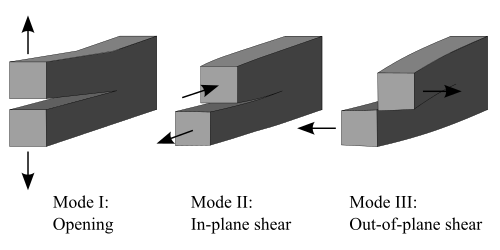
\includegraphics[width=0.75\textwidth]{fracture_modes}
  \caption{%
    The three independent fracture modes at a crack tip.
    Mode~I (opening): symmetric tensile loading perpendicular to the
    crack plane.
    Mode~II (in-plane shear): sliding of the crack faces parallel to the
    crack plane and perpendicular to the crack front.
    Mode~III (out-of-plane shear): tearing, with crack-face displacements
    parallel to the crack front.
    The general stress state is a superposition of all three, each weighted
    by its stress-intensity factor $K_I$, $K_{II}$, $K_{III}$.
  }
  \label{fig:fracture_modes}
\end{figure}

\section{Governing Equations: 2D Linear Elasticity}
\label{sec:elasticity}

The domain $\Omega \subset \R^2$ is occupied by a homogeneous, isotropic,
linearly elastic body under plane-strain conditions.
The displacement field $\bfu = (u_x, u_y)^T$ satisfies the Navier--Cauchy equations
\begin{equation}\label{eq:navier_cauchy}
  \begin{pmatrix}
    (\lambda+2\mu)\partial_{xx} + \mu\partial_{yy} & (\lambda+\mu)\partial_{xy} \\
    (\lambda+\mu)\partial_{xy} & \mu\partial_{xx} + (\lambda+2\mu)\partial_{yy}
  \end{pmatrix}
  \begin{pmatrix} u_x \\ u_y \end{pmatrix}
  = -\begin{pmatrix} f_x \\ f_y \end{pmatrix}
\end{equation}
in $\Omega$, subject to Dirichlet boundary conditions $\bfu = \bfg$ on $\dOmega$.
Here $\lambda$ and $\mu$ are the Lam\'{e} constants (material parameters) and
$\bff = (f_x, f_y)^T$ is the body force per unit volume.

The stress tensor and strain tensor for an isotropic material in plane strain are
\begin{align}
  \bfeps(\bfu) &= \tfrac{1}{2}\bigl(\nabla \bfu + (\nabla \bfu)^T\bigr),\\
  \bfsigma(\bfu) &= \lambda\,(\mathrm{tr}\,\bfeps)\,\mathbf{I}
                    + 2\mu\,\bfeps,
\end{align}
The von Mises equivalent stress is
\begin{equation}
  \sigma_\text{vm}
  = \sqrt{\sigma_{xx}^2 - \sigma_{xx}\sigma_{yy} + \sigma_{yy}^2 + 3\sigma_{xy}^2}.
\end{equation}

The Poisson ratio in plane strain and the Kolosov constant are
\begin{equation}
  \nu = \frac{\lambda}{2(\lambda+\mu)}, \qquad \kappa = 3 - 4\nu.
\end{equation}

\section{The Hierarchical Poincar\'{e}--Steklov (HPS) Algorithm}
\label{sec:hps}

A short description of the HPS algorithm~\cite{Martinsson2013,melia2025}
is given below for the scalar second-order elliptic boundary-value problem
\begin{equation}\label{eq:scalar_pde}
  \mathcal{L} u = f \quad \text{in } \Omega, \qquad u = g \quad \text{on } \dOmega.
\end{equation}
The method proceeds in three stages: local solve, merge (upward pass) and downward pass.

\subsection{Poincar\'{e}--Steklov operators}

A \emph{Poincar\'{e}--Steklov operator} $T: g \mapsto h$ maps one type of boundary data
to another for the equation $\mathcal{L}u = f$ on a subdomain.
The most common instance is the \emph{Dirichlet-to-Neumann} (DtN) map:
given Dirichlet data $g = u|_{\partial\Omega_j}$, it returns the outward normal derivative
$h = \partial_n u|_{\partial\Omega_j}$.
The key property exploited by the HPS algorithm is that these operators can be
\emph{merged}: the DtN operator for a composite domain $\Omega = \Omega_a \cup \Omega_b$
can be expressed purely in terms of the DtN operators of $\Omega_a$ and $\Omega_b$
via a Schur complement, without ever solving the PDE on the full domain.

Because $\mathcal{L}$ is linear, the solution decomposes as $u = v + w$, where
$v$ solves $\mathcal{L}v = f$ with zero Dirichlet data (particular solution) and
$w$ solves $\mathcal{L}w = 0$ with Dirichlet data $g$ (homogeneous solution).
The operator $T$ is therefore the DtN map for the homogeneous problem and both
$T^{(i)}$ and the associated particular-solution flux
$\mathbf{h}^{(i)} = \partial_n v^{(i)}|_{\partial\Omega_i}$
can be precomputed before the boundary data $g$ is known.

\subsection{Discretization}
\label{sec:discretization}

The domain $\Omega$ is recursively partitioned into a quadtree of depth $L$,
yielding $n_\text{leaves} = 4^L$ leaf patches.
\Cref{fig:chebyshev_grid} shows the two key grids for a simple two-dimensional
example with $L = 1$ and $p = 8$.
Each leaf is discretized on a $p \times p$ tensor-product Chebyshev--Lobatto
grid (panel~(a)), giving $p^2$ interior degrees of freedom per leaf and a total of
$N = 4^L p^2$ interior unknowns.
Leaf boundaries are discretized on $q$-point Gauss--Legendre grids with $q = p - 2$,
following~\cite{Gillman2015}.
Panel~(b) distinguishes the \emph{exterior} boundary points (blue circles, on
$\dOmega$) from the \emph{interior interface} points (red crosses, shared between
adjacent patches $\Omega_a, \Omega_b, \Omega_c, \Omega_d$); this distinction is
central to the merge step.

\begin{figure}[htbp]
  \centering
  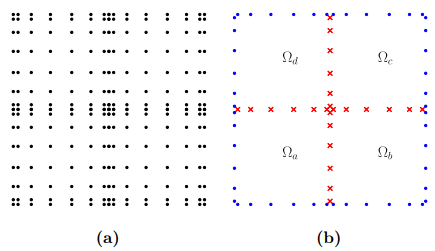
\includegraphics[width=0.8\textwidth]{chebyshev_grid}
  \caption{%
    High-order spectral collocation for a 2D problem with
    $p = 8$, $L = 1$.
    \textbf{(a)} Chebyshev--Lobatto interior points on all four leaves.
    \textbf{(b)} Gauss--Legendre boundary points: blue circles are exterior
    points on $\dOmega$; red crosses are interior interface points shared
    by adjacent patches $\Omega_a$, $\Omega_b$, $\Omega_c$, $\Omega_d$.
    (Figure adapted from~\protect\cite{melia2025}.)
  }
  \label{fig:chebyshev_grid}
\end{figure}

\subsection{Local solve stage}

On each leaf $i$, the spectral differentiation matrices are assembled into the
discrete operator $\mathbf{L}^{(i)} \in \R^{p^2 \times p^2}$.
A \emph{boundary-bordering} technique augments this system so that Dirichlet data
can be enforced along the leaf boundary while the PDE is collocated at all
interior Chebyshev nodes.
The bordered system is inverted once to extract:
\begin{itemize}
  \item $\mathbf{Y}^{(i)} \in \R^{p^2 \times q_\text{bdry}}$:
    the \emph{solution operator}, mapping any leaf boundary data to the
    corresponding homogeneous solution at interior Chebyshev nodes.
  \item $\mathbf{v}^{(i)} \in \R^{p^2}$: the particular solution at interior nodes.
\end{itemize}
Applying a fixed interpolation--differentiation operator to $\mathbf{Y}^{(i)}$ and
$\mathbf{v}^{(i)}$ yields the leaf-level DtN matrix $\mathbf{T}^{(i)}$ and the
particular-solution outgoing data $\mathbf{h}^{(i)}$.
This stage is \emph{embarrassingly parallel} across all $4^L$ leaves, and its cost
is $\mathcal{O}(p^6 n_\text{leaves})$ (dominated by the $p^2 \times p^2$ matrix
inversion on each leaf).

\subsection{Merge (upward pass) stage}

Starting from the leaves, the algorithm merges groups of four sibling nodes into
their parent until the root is reached.
Let $j$ be a parent node with children $\{a, b, c, d\}$.
Define index sets $\mathcal{E}$ (exterior boundary points of $j$, blue in
\cref{fig:chebyshev_grid}(b)) and $\mathcal{I}$ (interior interface points, red).
Using block notation, the DtN matrices of the children are assembled into
\begin{equation}\label{eq:block_system}
  \begin{bmatrix} A & B \\ C & D \end{bmatrix}
  \begin{bmatrix} \mathbf{g}_\mathcal{E} \\ \mathbf{g}_\mathcal{I} \end{bmatrix}
  = \begin{bmatrix}
      \mathbf{u}_\mathcal{E} - \mathbf{h}^{(\text{child})}_\mathcal{E} \\
      - \mathbf{h}^{(\text{child})}_\mathcal{I}
    \end{bmatrix},
\end{equation}
where $A, B, C, D$ are assembled blockwise from $\{\mathbf{T}^{(a)}, \mathbf{T}^{(b)},
\mathbf{T}^{(c)}, \mathbf{T}^{(d)}\}$ and the continuity conditions across merge
interfaces.
Since $\mathbf{g}_\mathcal{E}$ (the exterior boundary data of node $j$) is not yet
known, $\mathbf{g}_\mathcal{I}$ is eliminated via a Schur complement on $D$:
\begin{align}
  \mathbf{T}^{(j)} &= A - B D^{-1} C,
  \label{eq:T_merge}\\
  \mathbf{h}^{(j)} &= \mathbf{h}^{(\text{child})}_\mathcal{E}
                     - B D^{-1} \mathbf{h}^{(\text{child})}_\mathcal{I},
  \label{eq:h_merge}\\
  \mathbf{S}^{(j)} &= -D^{-1} C,
  \label{eq:S_merge}\\
  \tilde{\mathbf{g}}^{(j)} &= -D^{-1} \mathbf{h}^{(\text{child})}_\mathcal{I}.
  \label{eq:gtilde_merge}
\end{align}
Here $\mathbf{T}^{(j)}$ and $\mathbf{h}^{(j)}$ are passed to the next merge level;
$\mathbf{S}^{(j)}$ (the \emph{propagation operator}) and $\tilde{\mathbf{g}}^{(j)}$
(particular-solution data at the interior interfaces) are stored for the downward
pass.
The dominant cost at each level is inverting $D$, whose size grows as $\mathcal{O}(pq^{L-\ell})$
at level $\ell$; the total merge cost is $\mathcal{O}(p^3 n_\text{leaves}^{3/2})$ in 2D.

\subsection{Downward pass}

Once the boundary data $\mathbf{g}$ on $\dOmega$ is available, the precomputed
operators are applied in a single top-to-bottom sweep of the tree:
\begin{equation}
  \mathbf{g}^{(j)}_\mathcal{I} = \mathbf{S}^{(j)} \mathbf{g}^{(j)}_\mathcal{E}
  + \tilde{\mathbf{g}}^{(j)},
\end{equation}
propagating boundary data from each node to the boundaries of its children.
At the leaf level:
\begin{equation}
  \mathbf{u}^{(i)} = \mathbf{Y}^{(i)} \mathbf{g}^{(i)} + \mathbf{v}^{(i)}.
\end{equation}
The downward pass consists entirely of matrix-vector products with cost
$\mathcal{O}(p^2 n_\text{leaves})$, and it can be re-executed in negligible time
for new boundary data $\mathbf{g}$ or new sources $f$ (after recomputing only $\mathbf{v}^{(i)}$
and $\tilde{\mathbf{g}}^{(j)}$).

\subsection{Complexity summary}

The local solve stage costs $\mathcal{O}(p^6 n_\text{leaves})$ and is embarrassingly parallel over leaves.
The merge (upward pass) costs $\mathcal{O}(p^3 n_\text{leaves}^{3/2})$ with parallelism within each tree level.
The downward pass costs $\mathcal{O}(p^2 n_\text{leaves})$.
The build stage (local solve + merge) is performed \emph{once} per operator.
The downward pass is re-applied for each new right-hand side at a small cost, making
HPS highly efficient for problems requiring many solves with the same operator.

\section{ADI Splitting for Coupled Elasticity}
\label{sec:gs}

The Navier--Cauchy system \cref{eq:navier_cauchy} couples $u_x$ and $u_y$ through the
$(\lambda+\mu)\partial_{xy}$ off-diagonal terms, preventing direct use of the scalar
HPS solver.
The key observation is that if the coupling is treated as a known source, each component
satisfies a decoupled scalar elliptic equation of the form~\cref{eq:scalar_pde}. This
motivates an alternating fixed-point iteration.
At each step $k$, $u_x$ is solved first with the cross-derivative term from the
previous iterate $u_y^{(k-1)}$; then $u_y$ is solved using the updated $u_x^{(k)}$:
\begin{subequations}\label{eq:adi}
\begin{alignat}{2}
  \bigl[(\lambda+2\mu)\partial_{xx} + \mu\partial_{yy}\bigr]\,u_x^{(k)}
    &= -f_x - (\lambda+\mu)\,\partial_{xy}\,u_y^{(k-1)},
    &\quad u_x^{(k)}\big|_{\dOmega} &= g_x,
    \label{eq:solve_x}\\
  \bigl[\mu\partial_{xx} + (\lambda+2\mu)\partial_{yy}\bigr]\,u_y^{(k)}
    &= -f_y - (\lambda+\mu)\,\partial_{xy}\,u_x^{(k)},
    &\quad u_y^{(k)}\big|_{\dOmega} &= g_y.
    \label{eq:solve_y}
\end{alignat}
\end{subequations}
Each subproblem is a scalar elliptic boundary value problem to which HPS applies
directly.

\paragraph{Cost structure.}
Since the operator in each subproblem of \cref{eq:adi} is fixed across iterations,
\texttt{build\_solver} is called \emph{once} per displacement component,
storing the factored operators $\mathbf{Y}^{(i)},\mathbf{S}^{(j)},\mathbf{T}^{(j)}$.
Each ADI iteration then calls only the inexpensive \texttt{solve} (downward pass), plus
a batched spectral cross-derivative product at cost $\mathcal{O}(p^4 n_\text{leaves})$.
The assumption is that the ADI iteration converges in a small number of steps, independent
of the discretization size.

\paragraph{Convergence criterion.}
Iterations continue until the $\ell^\infty$ displacement update falls below
$\text{tol} = 10^{-14}$:
\begin{equation}
  \max_i \bigl(\|u_x^{(k)}-u_x^{(k-1)}\|_\infty + \|u_y^{(k)}-u_y^{(k-1)}\|_\infty\bigr) < \text{tol},
\end{equation}
ensuring iteration errors remain well below the discretization error for all
polynomial degrees tested.

\section{Case 1: Smooth Manufactured Solution}
\label{sec:results_smooth}

\subsection{Convergence}

The problem is solved on $\Omega = [-1,1]^2$ with $\lambda = \mu = 1$
and exact solution $u_x = \sin(\pi x)\sin(\pi y)$, $u_y = \cos(\pi x)\cos(\pi y)$,
with body forces $f_x = 2\mu\pi^2 \sin(\pi x)\sin(\pi y)$ and
$f_y = 2\mu\pi^2 \cos(\pi x)\cos(\pi y)$.
The sweep covers $p \in \{3, 4, 6, 8, 12, 16\}$ for $L \in \{2, 3, 4\}$.

\Cref{fig:elast2d_error} shows the relative $L^\infty$ error in $u_x$ and $u_y$
as a function of $p$ on a semi-log scale.
The curves demonstrate \emph{spectral-exponential}
convergence; errors reach double-precision ($\approx 10^{-13}$) at $p = 12$ for
$L \geq 3$.

\begin{figure}[htbp]
  \centering
  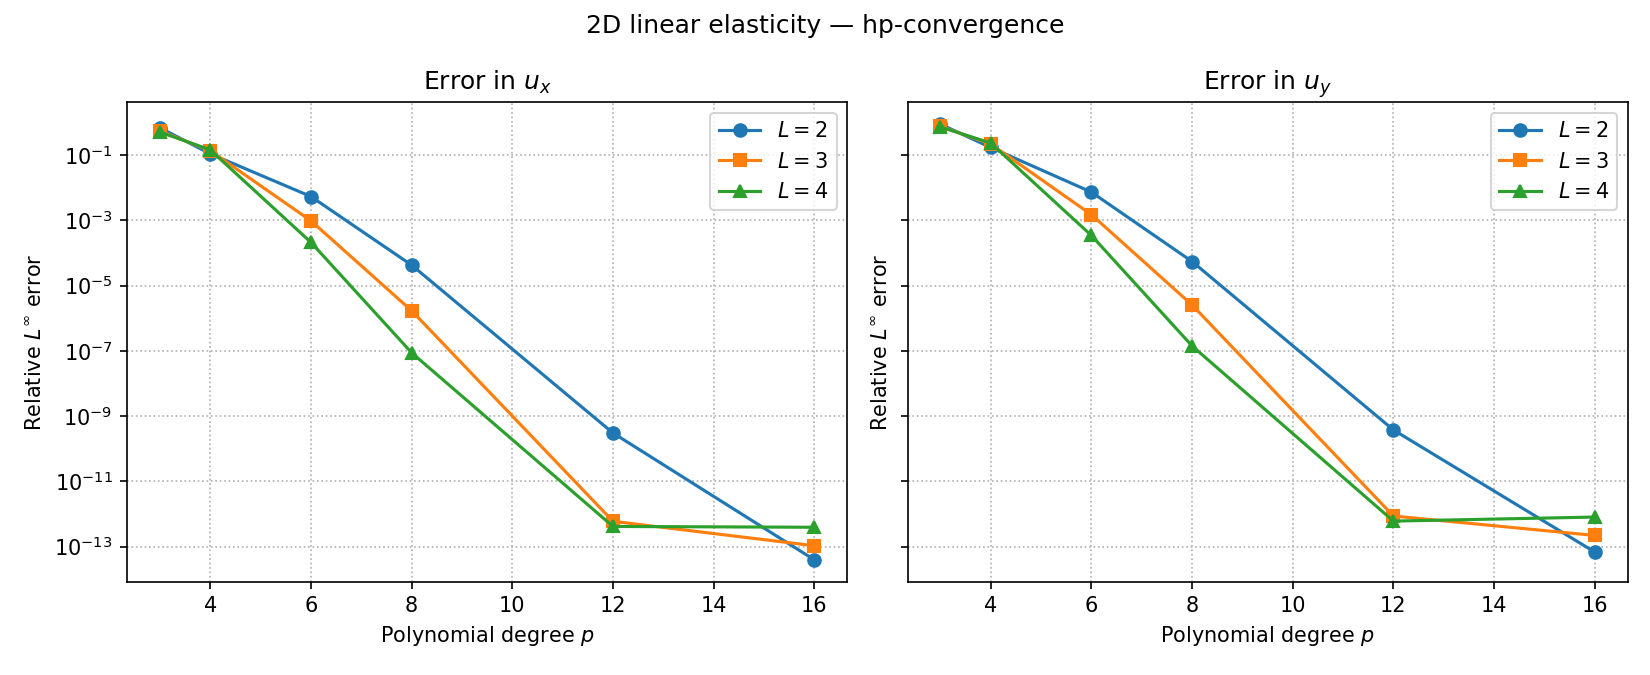
\includegraphics[width=\textwidth]{elast2d_error_vs_p}
  \caption{%
    Relative $L^\infty$ error vs.\ polynomial degree $p$ for the smooth
    manufactured solution on $[-1,1]^2$.
    Left: error in $u_x$; right: error in $u_y$.
    Each curve corresponds to a quadtree depth $L \in \{2,3,4\}$.
    Errors decay exponentially until double-precision saturation near $10^{-13}$.
  }
  \label{fig:elast2d_error}
\end{figure}

\subsection{Solution Fields and ADI Iterations}

\Cref{fig:elast2d_contours} shows displacement and pointwise absolute error at
$L=4$, $p=16$; all errors are at or below $5\times10^{-13}$.
For all $(p,L)$ tested, the ADI solver converged in fewer than 10 iterations,
essentially independent of $L$.

\begin{figure}[htbp]
  \centering
  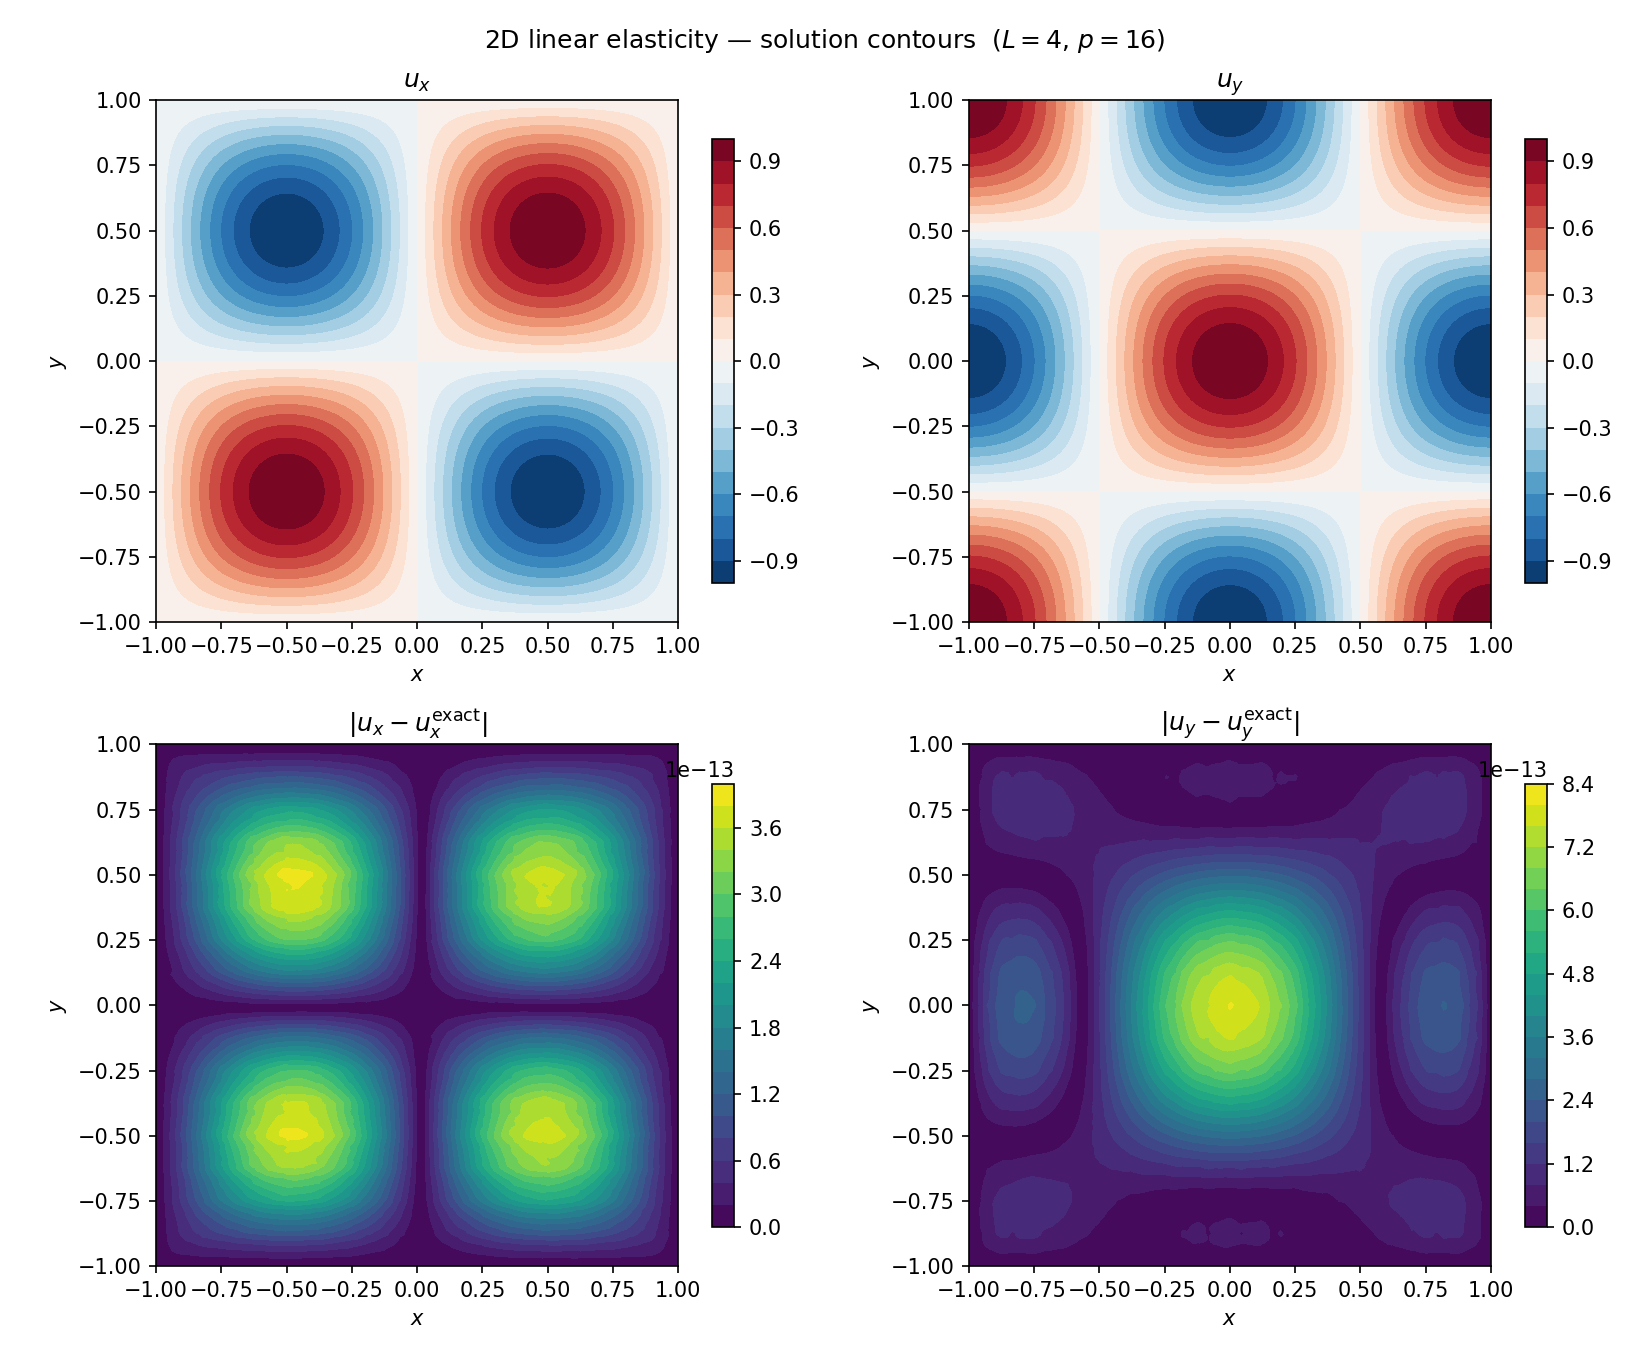
\includegraphics[width=\textwidth]{elast2d_solution_contours}
  \caption{%
    Numerical solution (top) and pointwise absolute error (bottom) for the
    smooth manufactured problem at $L=4$, $p=16$.
    Top left: $u_x$; top right: $u_y$.
    Bottom left: $|u_x - u_x^\text{exact}|$; bottom right: $|u_y - u_y^\text{exact}|$.
    All errors are at or below $5\times10^{-13}$.
  }
  \label{fig:elast2d_contours}
\end{figure}



\section{Case 2: Mode~I Crack-Tip Singularity}
\label{sec:results_crack}

\subsection{Problem Setup and Exact Solution}

For this mode-I crack-tip problem, the domain is $\Omega = [0,1]^2$,
with the crack tip at the corner $(0,0)$. The crack lies along the negative $x$-axis,
entirely outside $[0,1]^2$,
so the solution is single-valued in $\Omega$; however, the $\sqrt{r}$ behaviour
near the origin constitutes a corner singularity.

\Cref{fig:crack_tip_zone} illustrates the classical plastic zone surrounding a
Mode~I crack tip.
Inside this zone the material yields and the linear-elastic model breaks down. However,
this region is assumed to be small in this problem, so the linear-elastic solution is valid almost everywhere in $\Omega$.

\begin{figure}[htbp]
  \centering
  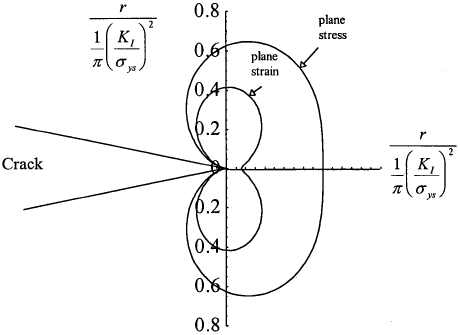
\includegraphics[width=0.45\textwidth]{crack_tip}
  \caption{%
    Irwin plastic zone for a Mode~I crack.
    The zone boundary for plane stress (outer curve) and plane strain (inner
    curve) are plotted in coordinates normalised by
    $r_p = \tfrac{1}{\pi}(K_I/\sigma_{ys})^2$.
  }
  \label{fig:crack_tip_zone}
\end{figure}

The exact solution is the Williams Mode~I asymptotic expansion~\cite{Williams1957}:
\begin{align}
  u_x &= \frac{K_I}{2\mu}\sqrt{\frac{r}{2\pi}}\cos\frac{\theta}{2}
          \bigl(\kappa - \cos\theta\bigr),
  \label{eq:williams_ux}\\
  u_y &= \frac{K_I}{2\mu}\sqrt{\frac{r}{2\pi}}\sin\frac{\theta}{2}
          \bigl(\kappa - \cos\theta\bigr),
  \label{eq:williams_uy}
\end{align}
with $r = \sqrt{x^2+y^2}$, $\theta = \mathrm{atan2}(y,x)$, Kolosov constant
$\kappa = 3-4\nu$, and $\nu = \lambda/(2(\lambda+\mu))$ the plane-strain
Poisson ratio.
Parameters are set to $\lambda = \mu = K_I = 1$, giving $\nu = 1/4$ and $\kappa = 2$.
The governing equations are \cref{eq:navier_cauchy} with $\mathbf{f} = \mathbf{0}$,
and Dirichlet data on all four sides of $[0,1]^2$ is set exactly to
\cref{eq:williams_ux,eq:williams_uy}.

\subsection{Convergence Results}

Because $\bfu \sim r^{1/2}$ near the origin (Sobolev regularity
$H^{3/2-\epsilon}$), best-approximation theory predicts algebraic convergence~\cite{BrennerScott}:
\begin{equation}
  \|u - u_p\|_{L^\infty} = \mathcal{O}(p^{-1/2}),
\end{equation}
independent of the mesh refinement level. This barrier is universal:
standard FEM shows the same rate (see \cref{fig:fem_convergence} in \cref{sec:appendix_fem}).

\Cref{fig:crack_error} shows the relative $L^\infty$ errors for the crack-tip
problem on a log-log scale, confirming the predicted algebraic rate $\mathcal{O}(p^{-1/2})$.
The error at $p = 16$, $L = 4$ remains above $1\%$, several orders of magnitude
above the machine-precision floor reached for the smooth problem.
Finer meshes (larger $L$) consistently reduce errors at fixed $p$ by
shrinking the corner patch, but do not improve the algebraic convergence rate.

\begin{figure}[htbp]
  \centering
  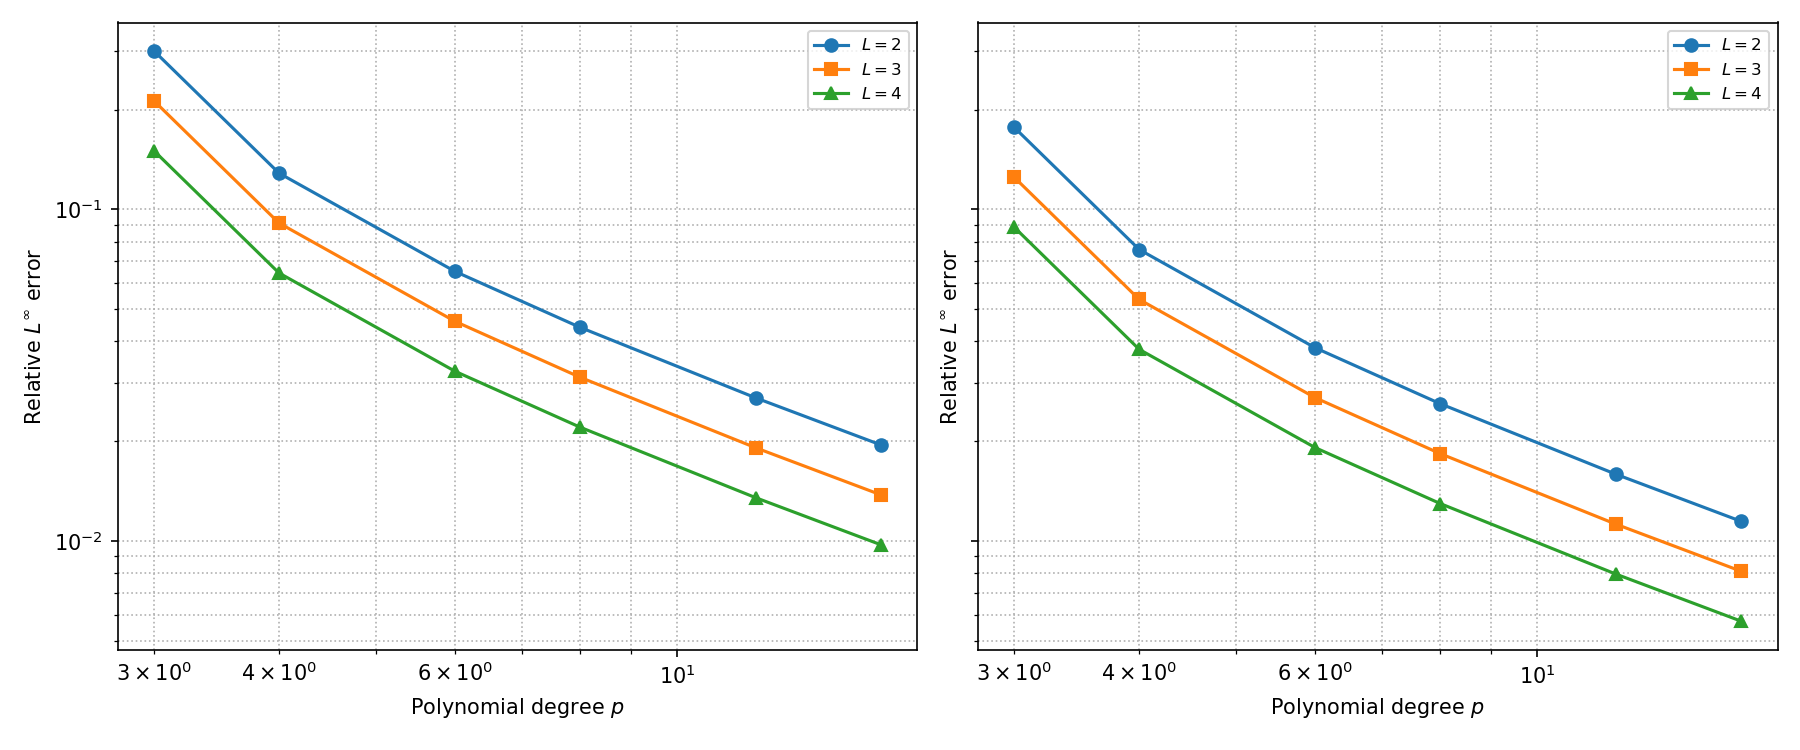
\includegraphics[width=\textwidth]{crack_error_vs_p}
  \caption{%
    Relative $L^\infty$ error vs.\ polynomial degree $p$ for the Mode~I
    crack-tip problem (log-log scale).
    Left: error in $u_x$; right: error in $u_y$.
    Convergence is algebraic at rate $\mathcal{O}(p^{-1/2})$. Increasing $L$
    reduces errors at fixed $p$ by shrinking the corner patch.
  }
  \label{fig:crack_error}
\end{figure}

\paragraph{Solution fields.}

\Cref{fig:crack_contours} shows the displacement components $u_x$ and $u_y$
at $L=4$, $p=16$; both fields radiate from the crack tip with the $\sqrt{r}$
growth of the Williams expansion.
\Cref{fig:crack_stress} shows the corresponding Cauchy stress components and
von Mises stress, all exhibiting the classical $1/\sqrt{r}$ singularity;
qualitative features match textbook fracture mechanics results.

\begin{figure}[htbp]
  \centering
  \begin{subfigure}[b]{\textwidth}
    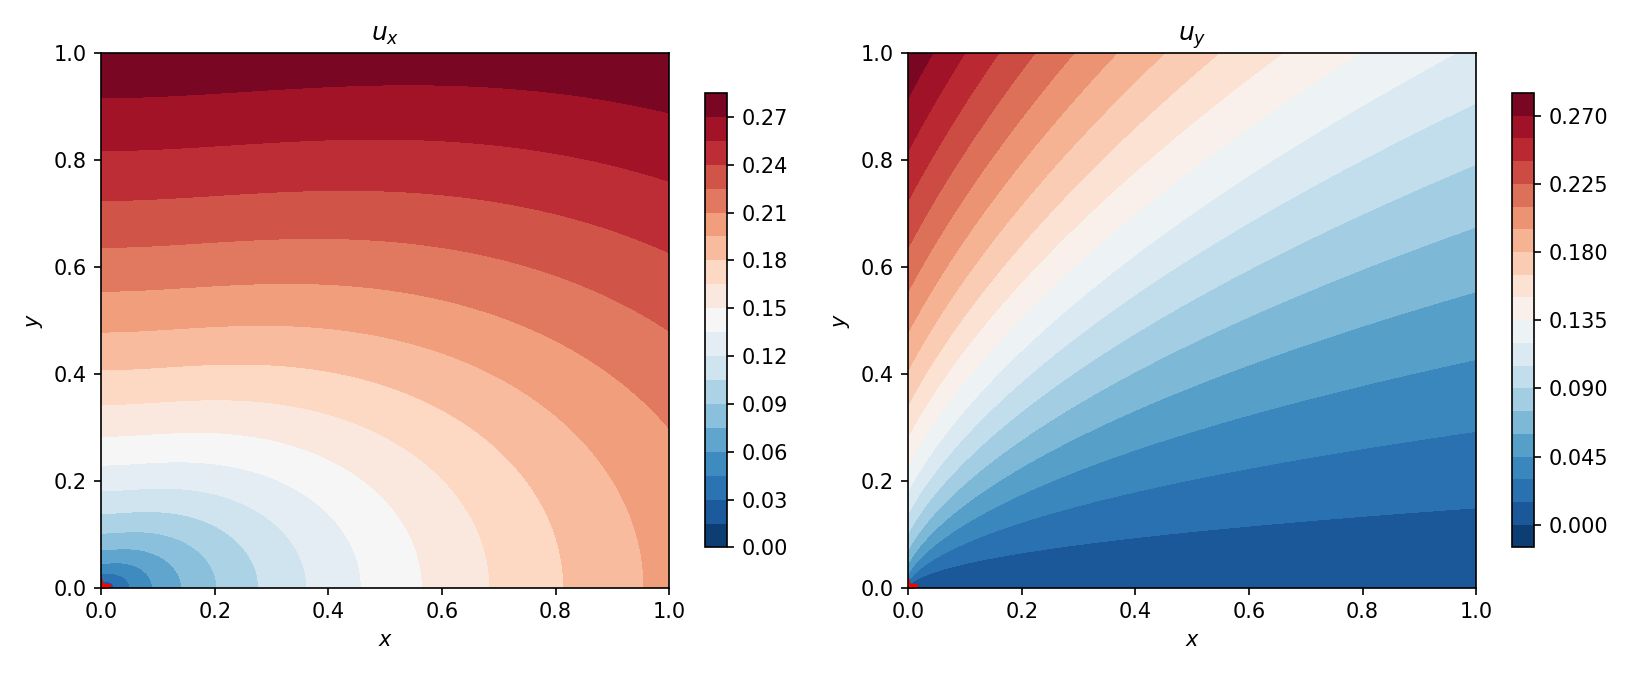
\includegraphics[width=\textwidth]{crack_solution_contours}
    \caption{%
      Displacement field.
      Left: $u_x$; right: $u_y$.
    }
    \label{fig:crack_contours}
  \end{subfigure}
  \\[1ex]
  \begin{subfigure}[b]{\textwidth}
    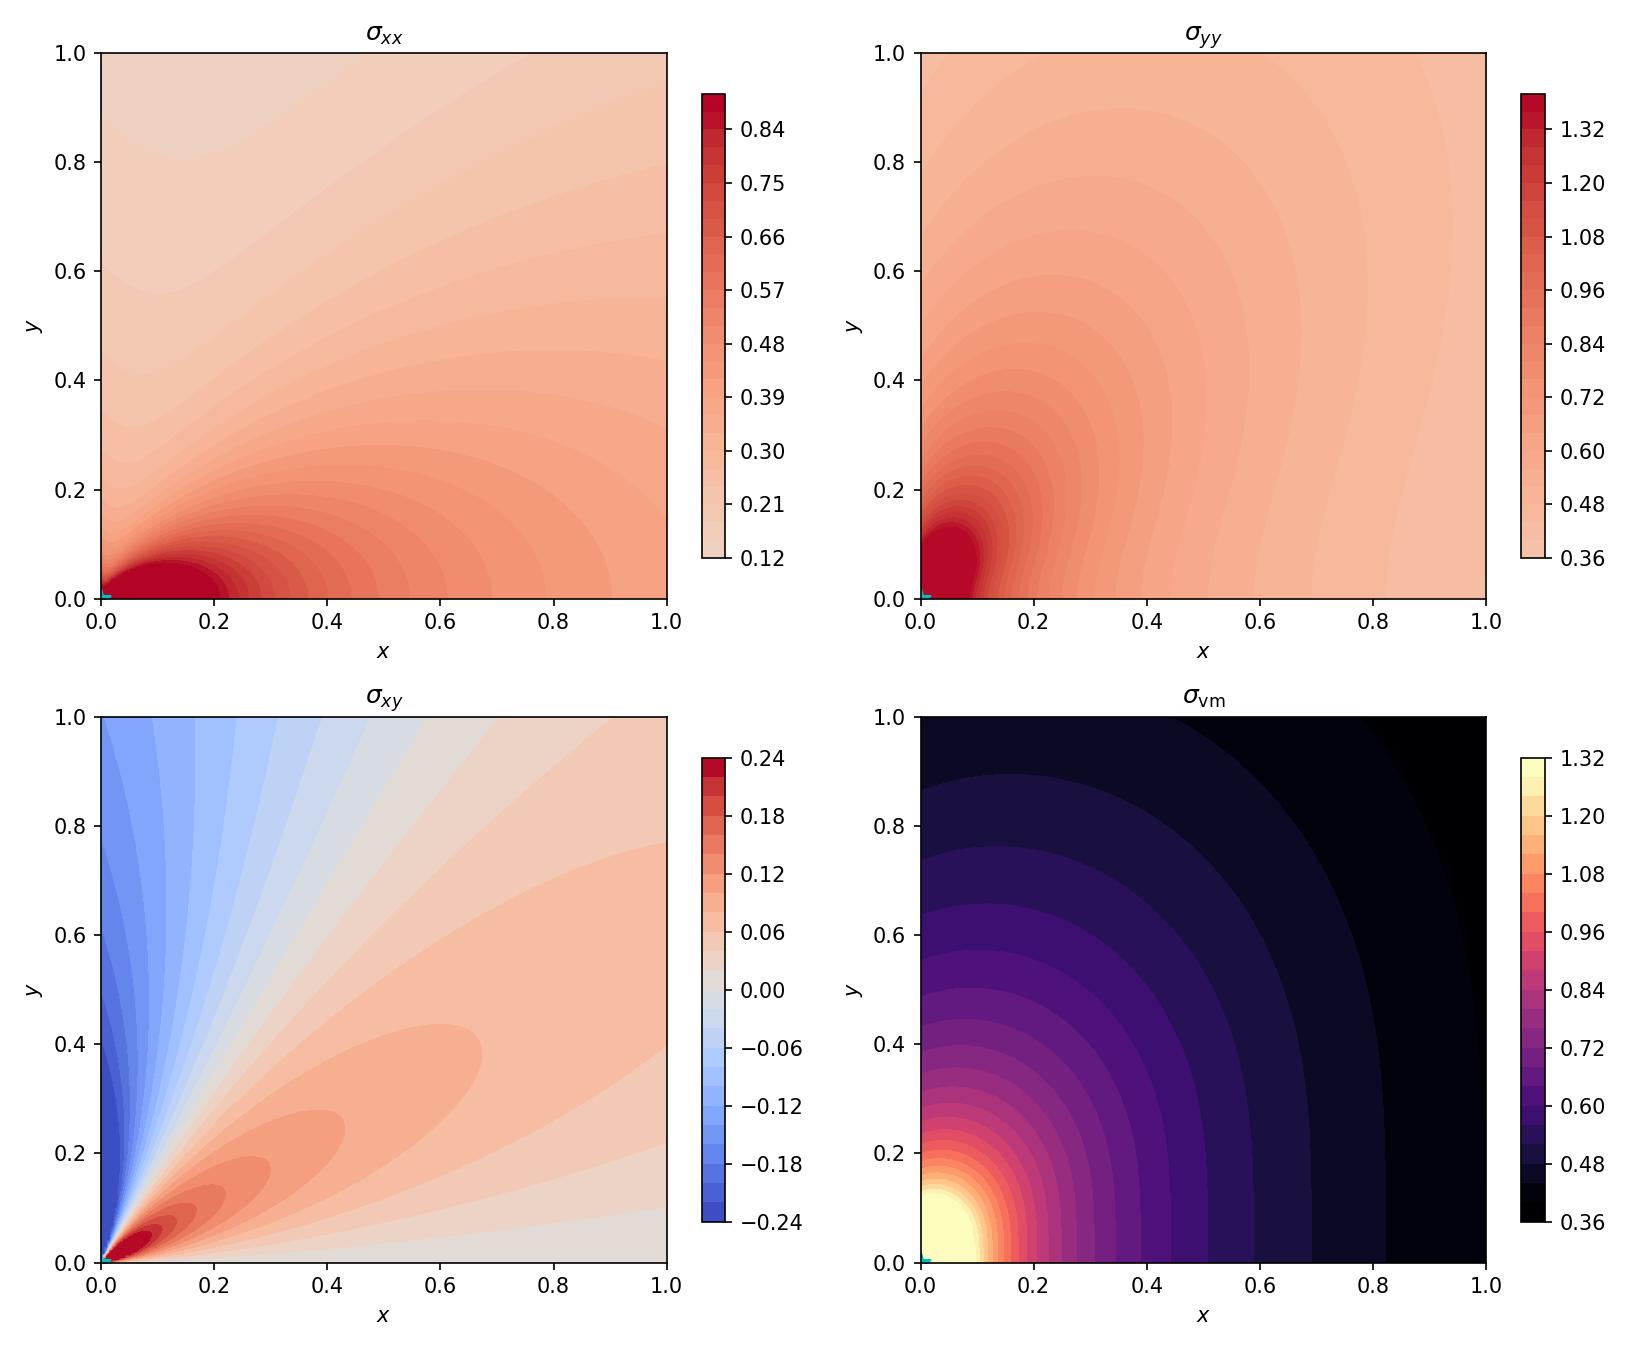
\includegraphics[width=\textwidth]{crack_stress_contours}
    \caption{%
      Stress fields.
      Top left: $\sigma_{xx}$; top right: $\sigma_{yy}$;
      bottom left: $\sigma_{xy}$; bottom right: $\sigma_\text{vm}$ (von Mises).
    }
    \label{fig:crack_stress}
  \end{subfigure}
  \caption{%
    Mode~I crack-tip solution fields at $L=4$, $p=16$.
  }
  \label{fig:crack_fields}
\end{figure}

\paragraph{ADI iteration count.}
With zero body force the right-hand side comes entirely from the cross-derivative
coupling term.
\Cref{fig:crack_iterations} shows the ADI iteration counts: the solver converges
in fewer than 20 iterations for all $p$ and $L$ tested, slightly more than the
smooth case because the singular $\sqrt{r}$ solution yields larger cross-derivative
values near the corner.

\begin{figure}[htbp]
  \centering
  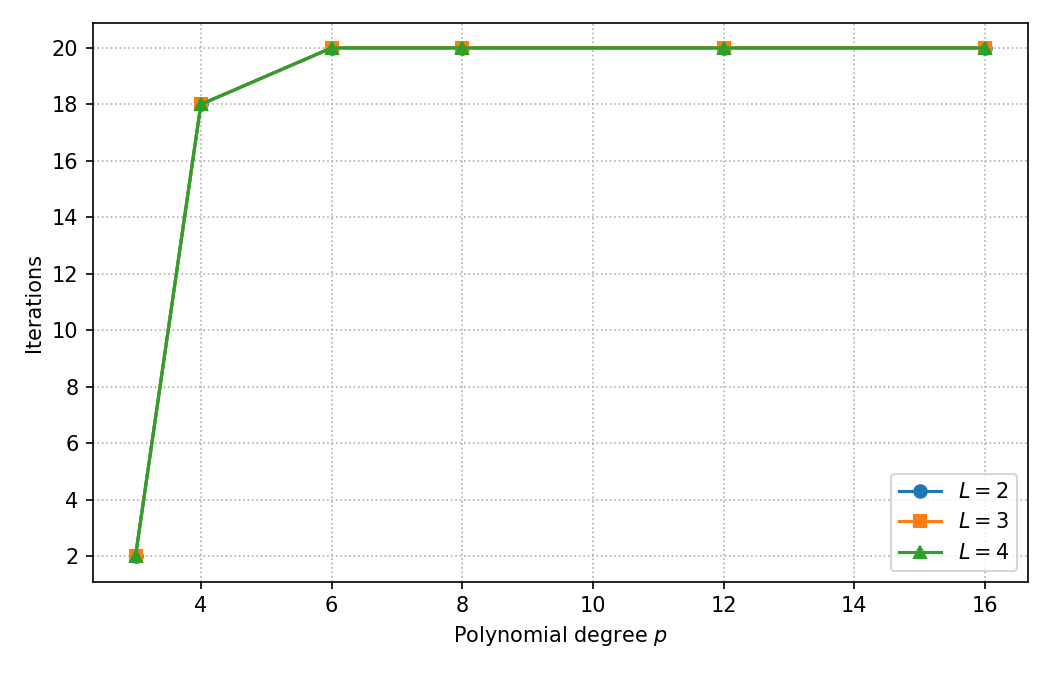
\includegraphics[width=0.65\textwidth]{crack_iterations}
  \caption{%
    ADI iteration counts for the Mode~I crack-tip problem as a function
    of $p$, for each $L \in \{2,3,4\}$.
  }
  \label{fig:crack_iterations}
\end{figure}

\subsection{Computational Cost}
\label{sec:cost}

\Cref{fig:runtimes} shows wall-clock time (build + solve) for both problems as a
function of $p$ and $L$. Run times increase with both $p$ and $L$, dominated by
the build stage. Both problems show nearly identical timing profiles; the slightly
larger ADI iteration count for the crack-tip case is negligible relative to the
build time.

\begin{figure}[htbp]
  \centering
  \begin{subfigure}[b]{0.48\textwidth}
    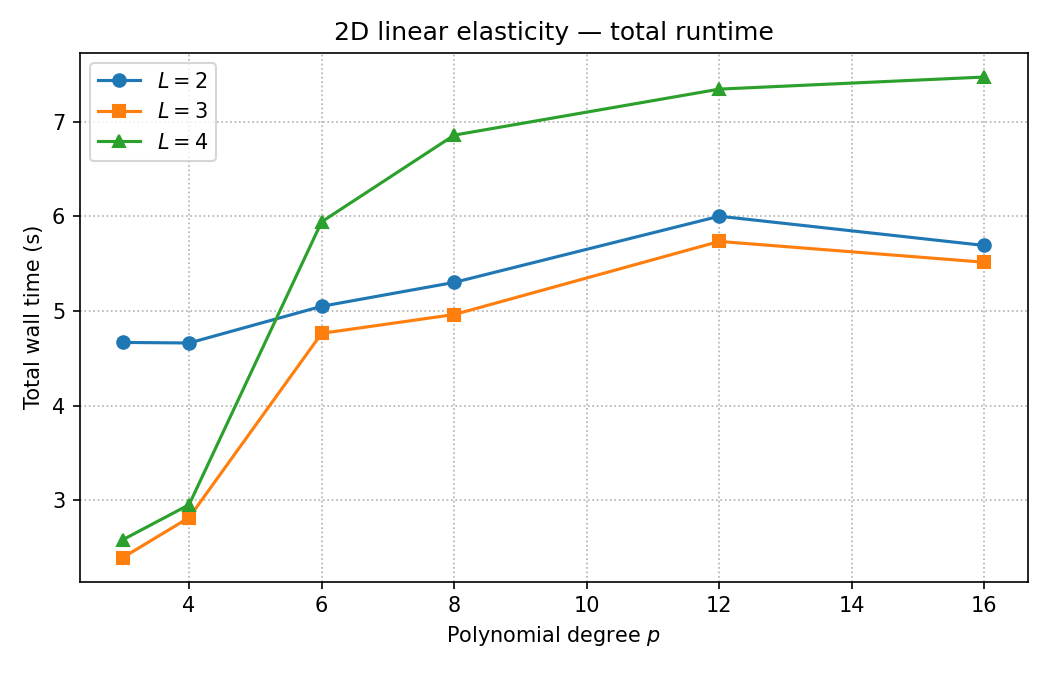
\includegraphics[width=\textwidth]{elast2d_runtimes}
    \caption{Smooth manufactured solution.}
    \label{fig:runtime_smooth}
  \end{subfigure}
  \hfill
  \begin{subfigure}[b]{0.48\textwidth}
    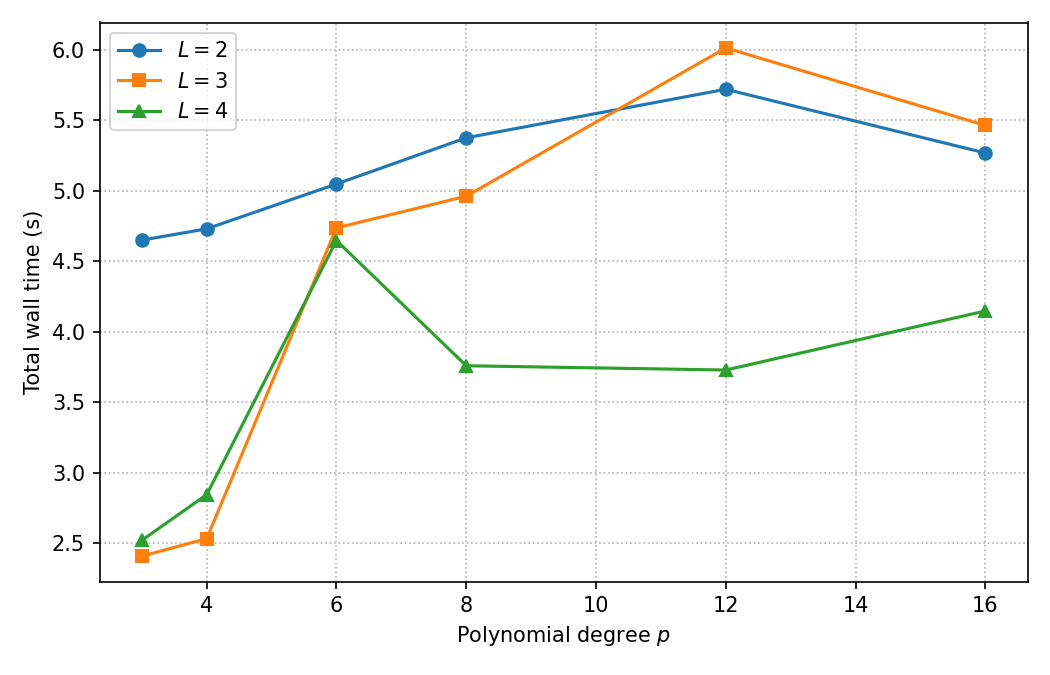
\includegraphics[width=\textwidth]{crack_runtimes}
    \caption{Mode~I crack-tip problem.}
    \label{fig:runtime_crack}
  \end{subfigure}
  \caption{%
    Total wall-clock time (build + solve) vs.\ polynomial degree $p$ for both
    benchmark problems, on a CPU.
    Run times increase with $p$ and $L$, dominated by the build stage.
  }
  \label{fig:runtimes}
\end{figure}

\section{Conclusions}
\label{sec:conclusions}

Results demonstrate that the HPS fast direct solver, combined with an ADI
splitting to handle the cross-derivative coupling in the Navier--Cauchy equations,
is a practical and efficient way to solve two-dimensional plane-strain linear
elasticity problems.

The key findings are:
\begin{enumerate}
  \item \textbf{Spectral-exponential convergence for smooth problems.}
    For the smooth manufactured solution, errors reach machine precision at
    moderate polynomial degrees ($p \approx 12$) regardless of the
    refinement level $L$, confirming the spectral accuracy of the composite
    Chebyshev collocation scheme.
  \item \textbf{Algebraic convergence for singular problems.}
    For the Mode~I crack-tip problem, convergence degrades to the theoretically
    predicted $\mathcal{O}(p^{-1/2})$ algebraic rate.
    Errors remain above $1\%$ even at $p = 16$, highlighting the fundamental
    limitation that corner singularities impose on polynomial approximation.
  \item \textbf{Efficient ADI splitting.}
    The ADI scheme converges in fewer than 10 iterations for the smooth problem
    and fewer than 20 for the singular problem, with the build stage executed
    only once per component.
\end{enumerate}

Directions for future work include:
\begin{itemize}
  \item \emph{Adaptive $h$-refinement} concentrated near the singularity;
    \texttt{jaxhps} already supports adaptive quadtree refinement, making this
    extension straightforward.
  \item GPU acceleration using the JAX backend of \texttt{jaxhps}~\cite{melia2025},
    which could enable much larger problem sizes and three-dimensional elasticity.
  \item The incompressible limit ($\nu \to 1/2$), where $\lambda \to \infty$
    strengthens the cross-derivative coupling.
  \item Other singularity types (e.g.\ material interfaces) and their impact on
    convergence.
\end{itemize}

\section*{Acknowledgments}
The numerical experiments in this report were carried out using
\texttt{jaxhps}~\cite{melia2025}, an open-source JAX implementation of the
hierarchical Poincar\'{e}--Steklov algorithm developed by Melia et al.
The library is publicly available at
\url{https://github.com/meliao/jaxhps}.

\bibliographystyle{siamplain}
\bibliography{references}

\appendix

\section{HPS Pseudocode}
\label{sec:appendix}

The three algorithmic stages of the HPS method are listed below in the notation
of \cref{sec:hps}, for the 2D DtN variant.  Full derivations are given
in~\cite{Martinsson2013,melia2025}.

\begin{algorithm}[H]
\caption{Local solve stage}
\label{alg:local}
\begin{algorithmic}[1]\small
  \STATE \textbf{Input:} $\{\mathbf{L}^{(i)}\}$, $\{\mathbf{f}^{(i)}\}$, differentiation matrices.
  \FOR{leaf $i = 1,\ldots,n_\text{leaves}$}
    \STATE Apply boundary bordering; invert bordered system
           $\;\triangleright$ \emph{cost $\mathcal{O}(p^6)$ per leaf}
    \STATE Extract $\mathbf{Y}^{(i)}$, $\mathbf{T}^{(i)}$, $\mathbf{v}^{(i)}$, $\mathbf{h}^{(i)}$
  \ENDFOR
  \STATE \textbf{Output:} $\{\mathbf{T}^{(i)},\mathbf{h}^{(i)},\mathbf{Y}^{(i)},\mathbf{v}^{(i)}\}$.
\end{algorithmic}
\end{algorithm}

\begin{algorithm}[H]
\caption{Merge (upward pass) stage}
\label{alg:merge}
\begin{algorithmic}[1]\small
  \STATE \textbf{Input:} $\{\mathbf{T}^{(i)},\mathbf{h}^{(i)}\}$ for all leaves.
  \FOR{level $\ell = L-1, \ldots, 0$}
    \FOR{node $j$ with children $a,b,c,d$}
      \STATE Assemble blocks $A,B,C,D$ from $\{\mathbf{T}^{(a)},\ldots,\mathbf{T}^{(d)}\}$ and child $\mathbf{h}$
      \STATE Invert $D$ $\;\triangleright$ \emph{main cost per level}
      \STATE $\mathbf{T}^{(j)} = A - BD^{-1}C$;\quad
             $\mathbf{h}^{(j)} = \mathbf{h}^{(\text{ch})}_\mathcal{E} - BD^{-1}\mathbf{h}^{(\text{ch})}_\mathcal{I}$
      \STATE $\mathbf{S}^{(j)} = -D^{-1}C$;\quad
             $\tilde{\mathbf{g}}^{(j)} = -D^{-1}\mathbf{h}^{(\text{ch})}_\mathcal{I}$
    \ENDFOR
  \ENDFOR
  \STATE \textbf{Output:} $\{\mathbf{S}^{(j)},\tilde{\mathbf{g}}^{(j)}\}$ for all interior nodes.
\end{algorithmic}
\end{algorithm}

\begin{algorithm}[H]
\caption{Downward pass (solve stage)}
\label{alg:down}
\begin{algorithmic}[1]\small
  \STATE \textbf{Input:} $\mathbf{g}|_{\partial\Omega}$;\; $\{\mathbf{S}^{(j)},\tilde{\mathbf{g}}^{(j)}\}$;\; $\{\mathbf{Y}^{(i)},\mathbf{v}^{(i)}\}$.
  \STATE $\mathbf{g}^{(\text{root})} \leftarrow \mathbf{g}|_{\partial\Omega}$
  \FOR{level $\ell = 0, \ldots, L-1$}
    \FOR{node $j$ with children $a,b,c,d$}
      \STATE $\mathbf{g}^{(j)}_\mathcal{I} = \mathbf{S}^{(j)}\mathbf{g}^{(j)}_\mathcal{E} + \tilde{\mathbf{g}}^{(j)}$;\quad distribute to children
    \ENDFOR
  \ENDFOR
  \FOR{leaf $i = 1,\ldots,n_\text{leaves}$}
    \STATE $\mathbf{u}^{(i)} = \mathbf{Y}^{(i)}\mathbf{g}^{(i)} + \mathbf{v}^{(i)}$
  \ENDFOR
  \STATE \textbf{Output:} $\{\mathbf{u}^{(i)}\}$.
\end{algorithmic}
\end{algorithm}

\section{FEM Convergence Reference}
\label{sec:appendix_fem}

For reference, \cref{fig:fem_convergence} shows the convergence of a standard Continuous
Galerkin FEM discretization on a uniform mesh.

\begin{figure}[htbp]
  \centering
  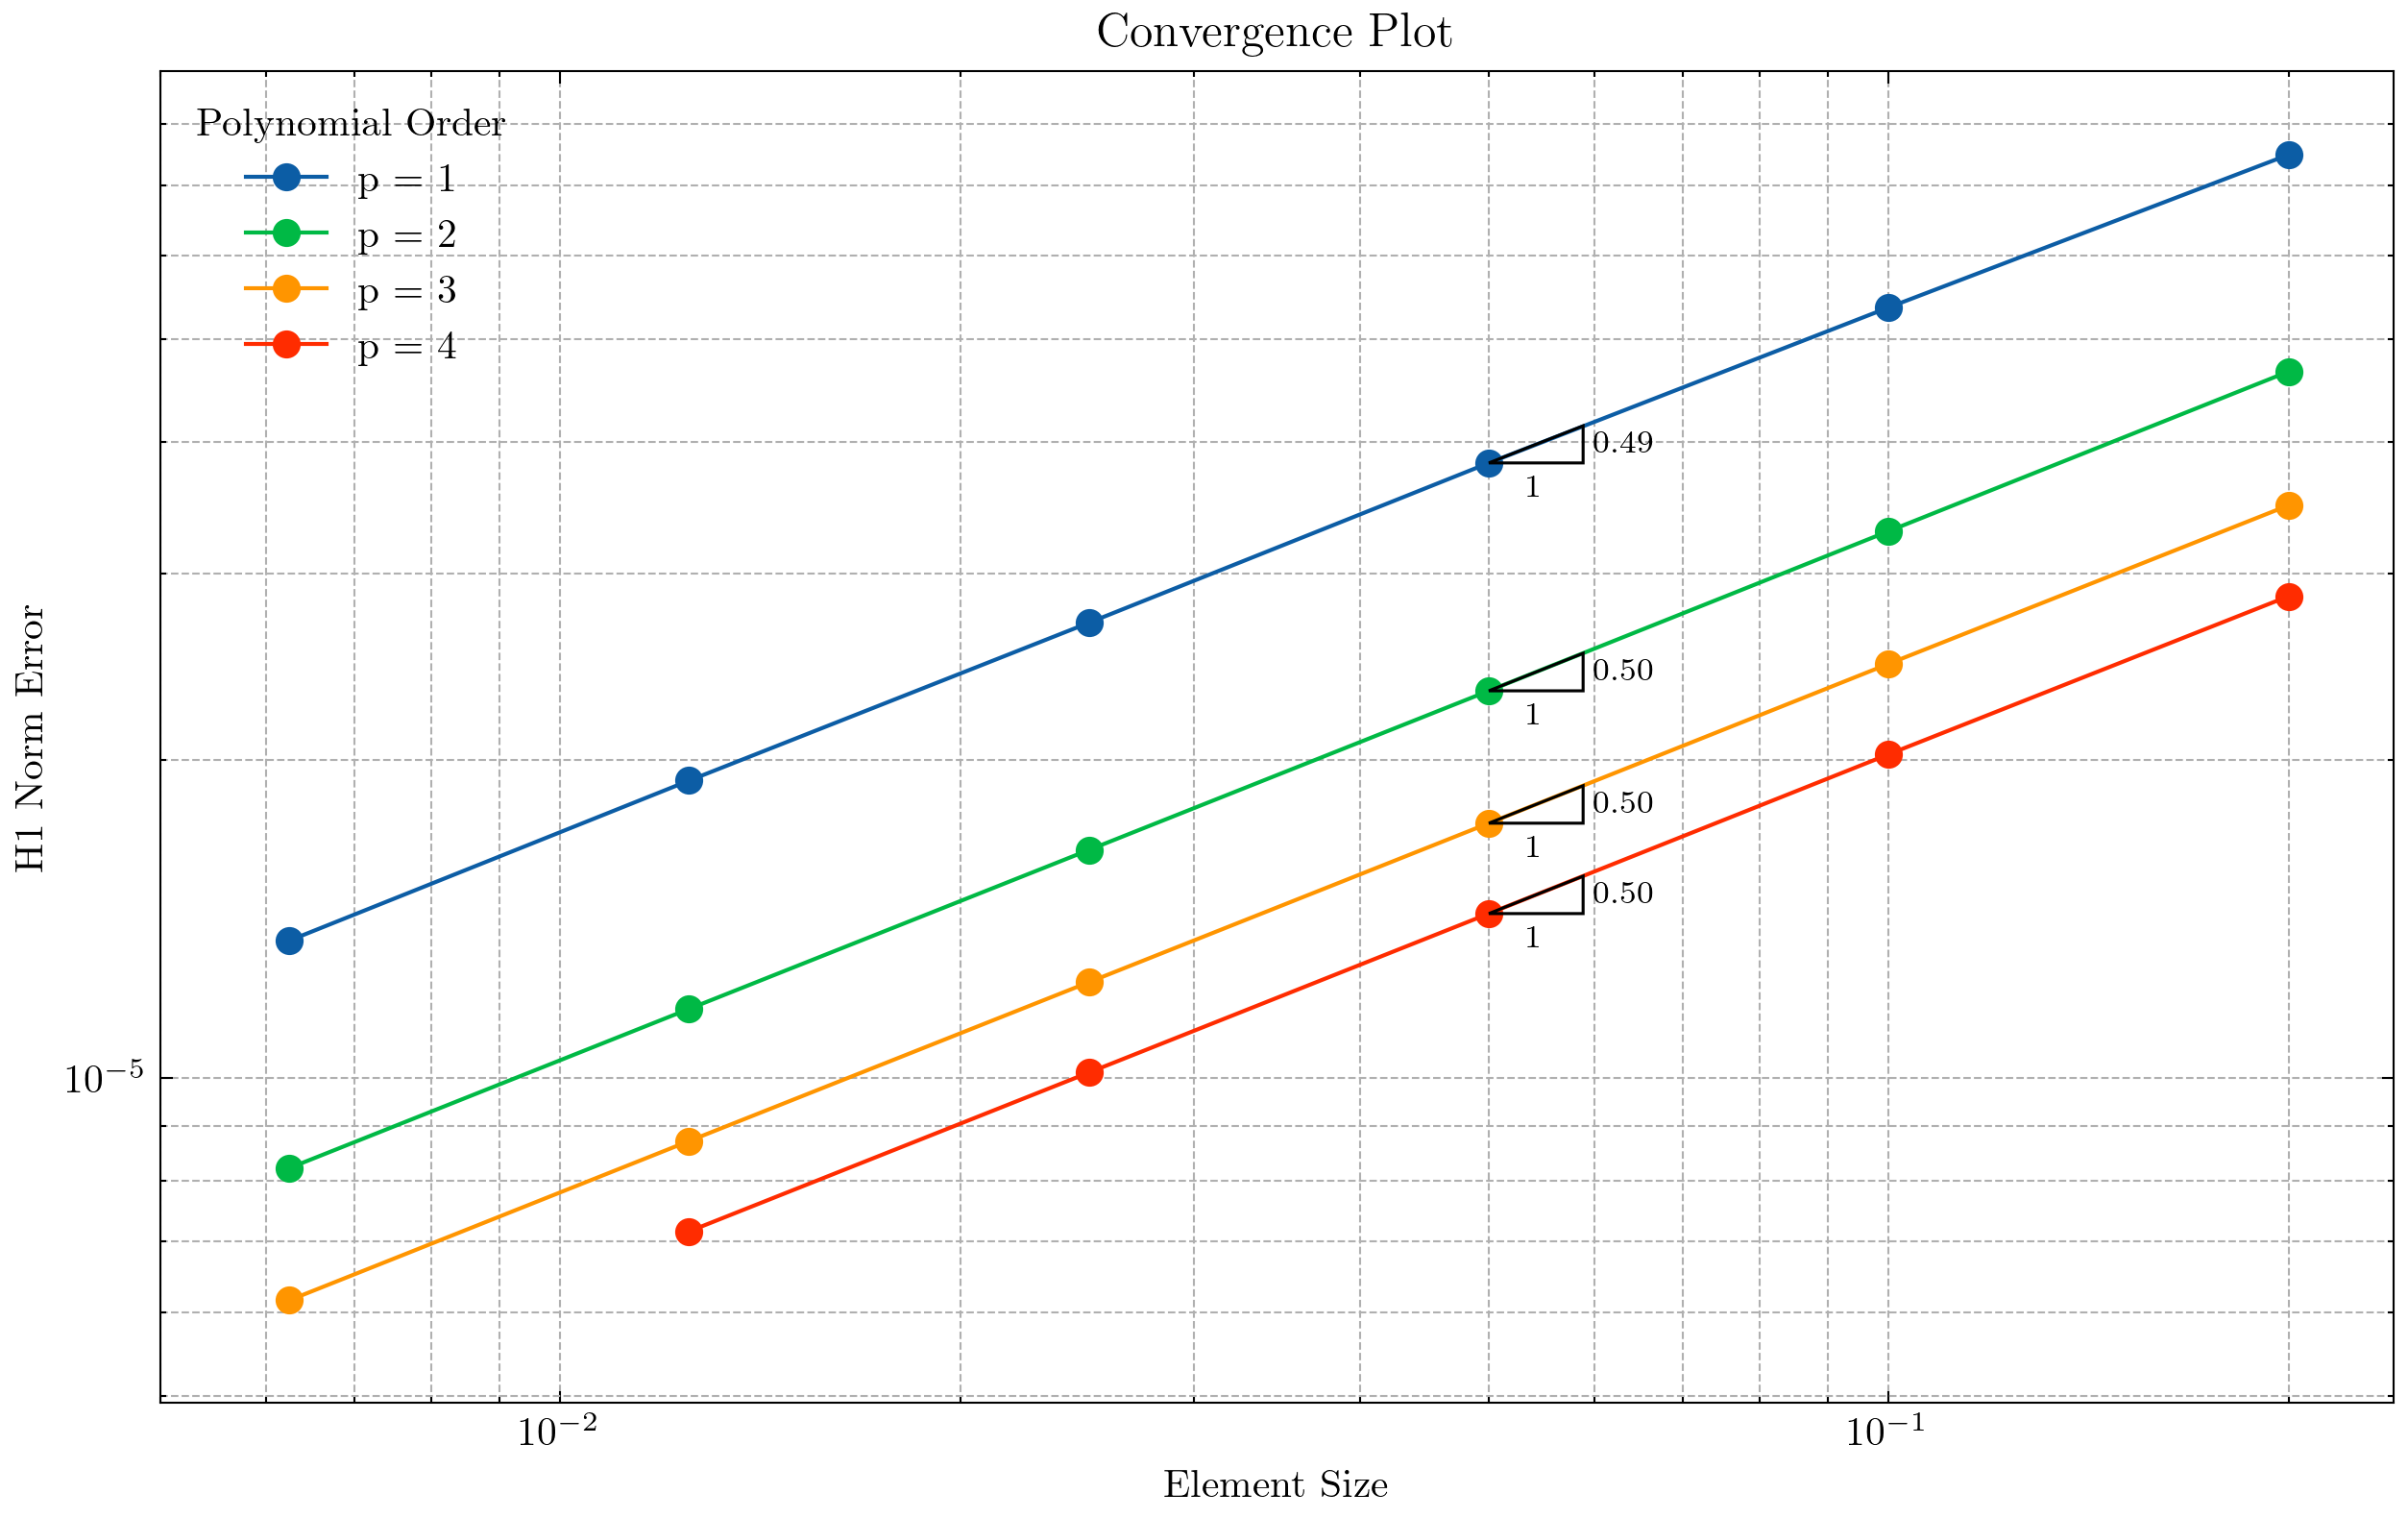
\includegraphics[width=0.8\textwidth]{convergence_plot_fem}
  \caption{%
    Continuous Galerkin FEM convergence in the $H^1$ norm for the Mode~I crack-tip
    problem. Polynomial orders $p = 1,\ldots,4$ all yield slope $\approx 0.5$ on the
    log-log scale, confirming the algebraic $\mathcal{O}(h^{1/2})$ rate imposed
    by the $\sqrt{r}$ singularity; higher $p$ reduces the constant but not the
    slope.
  }
  \label{fig:fem_convergence}
\end{figure}

\end{document}